\documentclass[runningheads,a4paper]{llncs}
\usepackage[utf8]{inputenc}
% linewrap symbol
\usepackage{color}

\def\baselinestretch{0.98}

\definecolor{grey}{RGB}{160,160,160}
\newcommand{\linewrap}{\raisebox{-.6ex}{\textcolor{grey}{$\hookleftarrow$}}}

% proper encoding
\usepackage[T1]{fontenc}

\usepackage{flushend}
\usepackage{verbatim} 

\usepackage{textcomp}
\usepackage{listings}
\lstset{frame=lines,captionpos=b,numberbychapter=false,escapechar=§,basicstyle=\ttfamily,upquote=true}

% todo macro
\usepackage{color}
\newcommand{\todo}[1]{\noindent\textcolor{red}{{\bf \{ToDo: }#1{\bf \}}}}

\usepackage{times}
%\usepackage{epsfig}
\usepackage{graphicx}
\usepackage{amsmath}
\usepackage{amssymb}
\usepackage{subfig}

% Thanks, http://lenaherrmann.net/2010/05/20/javascript-syntax-highlighting-in-the-latex-listings-package
\usepackage{color}
\definecolor{darkgray}{rgb}{.4,.4,.4}

\lstdefinelanguage{JavaScript}{
  keywords={push, typeof, new, true, false, catch, function, return, null, catch, switch, var, if, in, while, do, else, case, break},
  keywordstyle=\bfseries,
  ndkeywords={class, export, boolean, throw, implements, import, this},
  ndkeywordstyle=\color{darkgray}\bfseries,
  identifierstyle=\color{black},
  sensitive=false,
  comment=[l]{//},
  morecomment=[s]{/*}{*/},
  commentstyle=\color{darkgray},
  stringstyle=\color{red},
  morestring=[b]',
  morestring=[b]"
}

% If you comment hyperref and then uncomment it, you should delete
% egpaper.aux before re-running latex.  (Or just hit 'q' on the first latex
% run, let it finish, and you should be clear).
\usepackage{hyperref}
\def\sectionautorefname{Section}

\begin{document}

\mainmatter

\title{Please try this at home: yes, those reviews blend!}

% a short form should be given in case it is too long for the running head
\titlerunning{Please try this at home: yes, those reviews blend!}

% the name(s) of the author(s) follow(s) next
%
% NB: Chinese authors should write their first names(s) in front of
% their surnames. This ensures that the names appear correctly in
% the running heads and the author index.
%
\author{Thomas Steiner$^{1}$ \and Maribel Acosta$^{2}$ \and Ke Tao$^{3}$ \and Seth van Hooland$^{4}$}
\institute{Universitat Polit\'ecnica de Catalunya -- Department LSI, 08034 Barcelona, Spain\\
\urldef{\emails}\path|tsteiner@lsi.upc.edu|\emails
\and Simon Bolivar University, Bolivarian Republic of Venezuela\\
\urldef{\emails}\path|macosta@ldc.usb.ve|\emails
\and  Web Information Systems, TU Delft. PO Box 5031, 2600 GA Delft, the Netherlands\\
\urldef{\emails}\path|k.tao@tudelft.nl|\emails
\and Université Libre de Bruxelles, Belgium\\
\urldef{\emails}\path|svhoolan@ulb.ac.be|\emails
}
%
\authorrunning{Please try this at home: yes, those reviews blend!}
% (feature abused for this document to repeat the title also on left hand pages)

\maketitle
% \thispagestyle{empty}

%%%%%%%%% BODY TEXT
\section{Introduction and Motivation}
In 2007, the Internet marketing research company comScore examined~\cite{comscore2007} the impact of consumer-generated online reviews on offline sales for (amongst others) hotels. 24 percent of Internet users reported using online reviews prior to paying for a service delivered offline. Of those who consulted an online hotel review, 40 percent subsequently stayed at a reviewed hotel. 87 percent of hotel review users reported that the review had a significant influence on their choice of accommodation. In~\cite{chicagolaw2005}, Sunstein describes the process of spontaneous and planned group polarization, \emph{i.e.}, the process by which like-minded people go to extremes. He differentiates between planned and spontaneous polarization processes, where for the prior individuals or groups consciously try to pull others in their direction of thought, and where for the latter polarization just happens unplanned. For online reviews, this process can be observed when unhappy reviewers after reading other reviewers' reviews---and also oftentimes protected by their anonymity---leave less friendly reviews than they would have left in isolation. Big review websites typically have a paragraph on conflicts of interest in their user guidelines\footnote{For example, \url{http://www.yelp.com/guidelines}} where they prohibit businesses and their employees to write reviews about themselves or their competition. For the hotel sector there are many different sources for reviews, ranging from commercial hotel aggregation websites, to non-commercial travel portals. Travelers interested in a certain hotel are well-advised to check a hotel on several sources prior to a reservation. While many hotel review sites allow users to rate specific aspects of hotels, such as location, staff friendliness, or cleanness, oftentimes more value lies in knowledge about aspects that are not part of rating schemes: is the hotel's Wi-Fi darn slow? Does the hotel assign non-smokers smoking rooms? Is the \emph{chef de la cuisine} famous for his oysters? In this demonstration paper, with ReviewBlender\texttrademark \  we report on a Web browser extension\footnote{Google Chrome extension available at \url{http://tomayac.de/ReviewBlender.crx}} that facilitates the time-consuming task of summarizing reviews from different sources for the domain of hotel reviews on-the-fly. We therefore match hotels from different websites, perform named entity extraction and disambiguation followed by sentiment analysis on hotel reviews, and finally present the user with the consolidated hotel highlights and pain points in form of an easy to grasp tag cloud.

\section{Related Work}
As a result of the ever-growing impact of online reviews, there has been a trend towards systems to summarize and make sense of online reviews and to display them in an easily graspable way. Sentiment analysis plays a key role in this process. \cite{pang2008} by Bang and Lee provides an overview on techniques and approaches that promise to directly enable opinion-oriented information-seeking systems. In~\cite{blairgoldensohn2011}, Blair-Goldensohn \emph{et al.} describe a system for summarizing sentiments for local services including aspect extraction. Aspect extraction is the process of determining what aspects of a reviewed item reviewers write about. In~\cite{hu2004}, Hu and Liu demonstrate several techniques to achieve aspect extraction in the context of consumer reviews.

\section{Implementation Details}
\paragraph{Browser Extension Background}
Our Web browser extension is currently targeted to the Google Chrome browser. Chrome extensions are small software programs that users can install to enrich their browsing experience. They are written using a combination of standard Web technologies, such as HTML, JavaScript, and CSS. There are several types of extensions; for this paper we focus on extensions based on so-called \emph{content scripts}. Content scripts are JavaScript programs that run in the context of Web pages via dynamic code injection and thus can modify details of Web pages.

\paragraph{Hotel Matching on Different Websites}
We currently focus on the hotels.com hotel aggregation website with the extension, albeit the method is generalizable, however, needs some customization to each target website. Our browser extension gets triggered when the user navigates to the review tab on an individual hotel landing page. We extract the review texts via CSS selectors, which is brittleness-wise equivalent to screen scraping, however, the only way to access information across different websites that do not provide APIs. We match hotels on different websites using their names and their geocoded addresses. Geocoding is the process of finding associated latitude and longitude values from street addresses. If the hotel name of a supposedly matching hotel on two different websites matches, and if the geographic distance between to (latitude, longitude) points is less than a certain threshold, we consider the hotels the same.

\paragraph{Named Entity Extraction and Disambiguation, and Sentiment Analysis}
At this stage, we do not perform the tasks of named entity extraction and disambiguation, and sentiment analysis ourselves, but rather use Web services from AlchemyAPI~\cite{alchemyapi2011}. Their entity extraction API disambiguates extracted named entities from review texts and represents the named entities by URIs in the Linked Open Data cloud\footnote{\url{http://lod-cloud.net/}}. Their sentiment analysis API is in some cases able to detect the nature of the mention of a named entity (positive, neutral, negative), and in all cases detects the nature of the whole review text.

\paragraph{Tag Cloud Generation}
We count occurrences of named entities in all three sentiment categories (positive, neutral, negative). If one reviewer talks about the ``wireless network'' and another reviewer talks about the ``Wi-Fi'', then this would be counted as two occurrences of the same named entity represented by the URI \url{http://dbpedia.org/resource/Wireless_network}. \autoref{fig:blender} shows a sample tag cloud for the Las Vegas Luxor Hotel and Casino, where people are especially upset about the hotel's own Starbucks prices and service.

\vspace{-5mm}
\begin{figure}[h]
  \begin{center}
\subfloat[Placeholder during named entity extraction / disambiguation, and sentiment analysis.]{\label{fig:blender-a}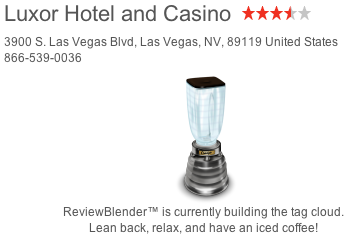
\includegraphics[width=0.35\textwidth]{./resources/blender}}
\hspace{10pt}
\subfloat[Disambiguated named entities and color-coded sentiments towards them.]{\label{fig:blender-b}\raisebox{13.25mm}{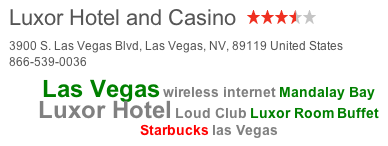
\includegraphics[width=0.35\textwidth]{./resources/tagcloud}}}
  \caption{The ReviewBlender\texttrademark \ before and after blending online reviews for a hotel.}
  \label{fig:blender}
  \end{center}  
\end{figure}

\vspace{-5mm}
\section{Future Work and Conclusion}
\todo{Bullshit about Future Work and Conclusion}

% back to normal size Computer Modern for URLs in bibliography
\renewcommand{\ttdefault}{cmvtt}
\renewcommand\UrlFont\tt

\bibliographystyle{splncs03}
\bibliography{sdow2011}

\end{document}